\chapter{A framework for Media Architectural Interfaces (MAIs)}
\label{chapterlabel4}

\section*{Chapter summary}

In this chapter, I develop a framework that outlines the requirements for media architecture to become interactive and accessible for people. The framework will be supported by a taxonomy that itemizes existing projects. Being aware of the framework will help designers clarify the nature of interaction they want to design for.  

\newpage


\section{ Media Architectural Interfaces (MAI) }

The terms Ad-hoc frameworks vs observational frameworks need to be researched again:
%Michelis, D., & Müller, J. (2011). The Audience Funnel: Observations of Gesture Based Interaction With Multiple Large Displays in a City Center. International Journal of Human-Computer Interaction, 27(6), 562–579. doi:10.1080/10447318.2011.555299

From considering the different types of electronic surfaces utilised in urban media art projects in the CC Network initiatives (section 2.3.1 table 2.1), we identify a particular form of interactive systems that enables engagement with space inhabitants. 
This we refer to as Media Architectural Interfaces (MAI).
MAI describe an ecology of tangible and non-tangible interfaces in a given context. 
They can be considered as interactive systems in urban space, which potentially entice people to step out of their habitual routine and perceive urban space through a new lens or act differently within it. 
In more detail, we consider MAI as the synthesis of situated and shared \textit{Interfaces}, which mediate participants’ engagement with large programmable electronic \textit{Surfaces} such as Urban Screens, Media Facades or Media Architecture in a given socio-spatial \textit{Context} (\label{fig:MAI_Framework}). 
Tangible interfaces are generally located on street level, whereas the electronic surfaces, which are connected to the tangible interface, are mostly vertical and attached to buildings or are the buildings themselves such as the case with Media Facades. 
Eventually they may disrupt movement and behavioural patterns in the given spatial setting (i.e. \textit{Context}). 
These \textit{Interfaces} call for explicit and shared interactions following the urbanHCI framework, specifying different interaction spaces within which people perform different activities.

\begin{figure}[htp]
\centering
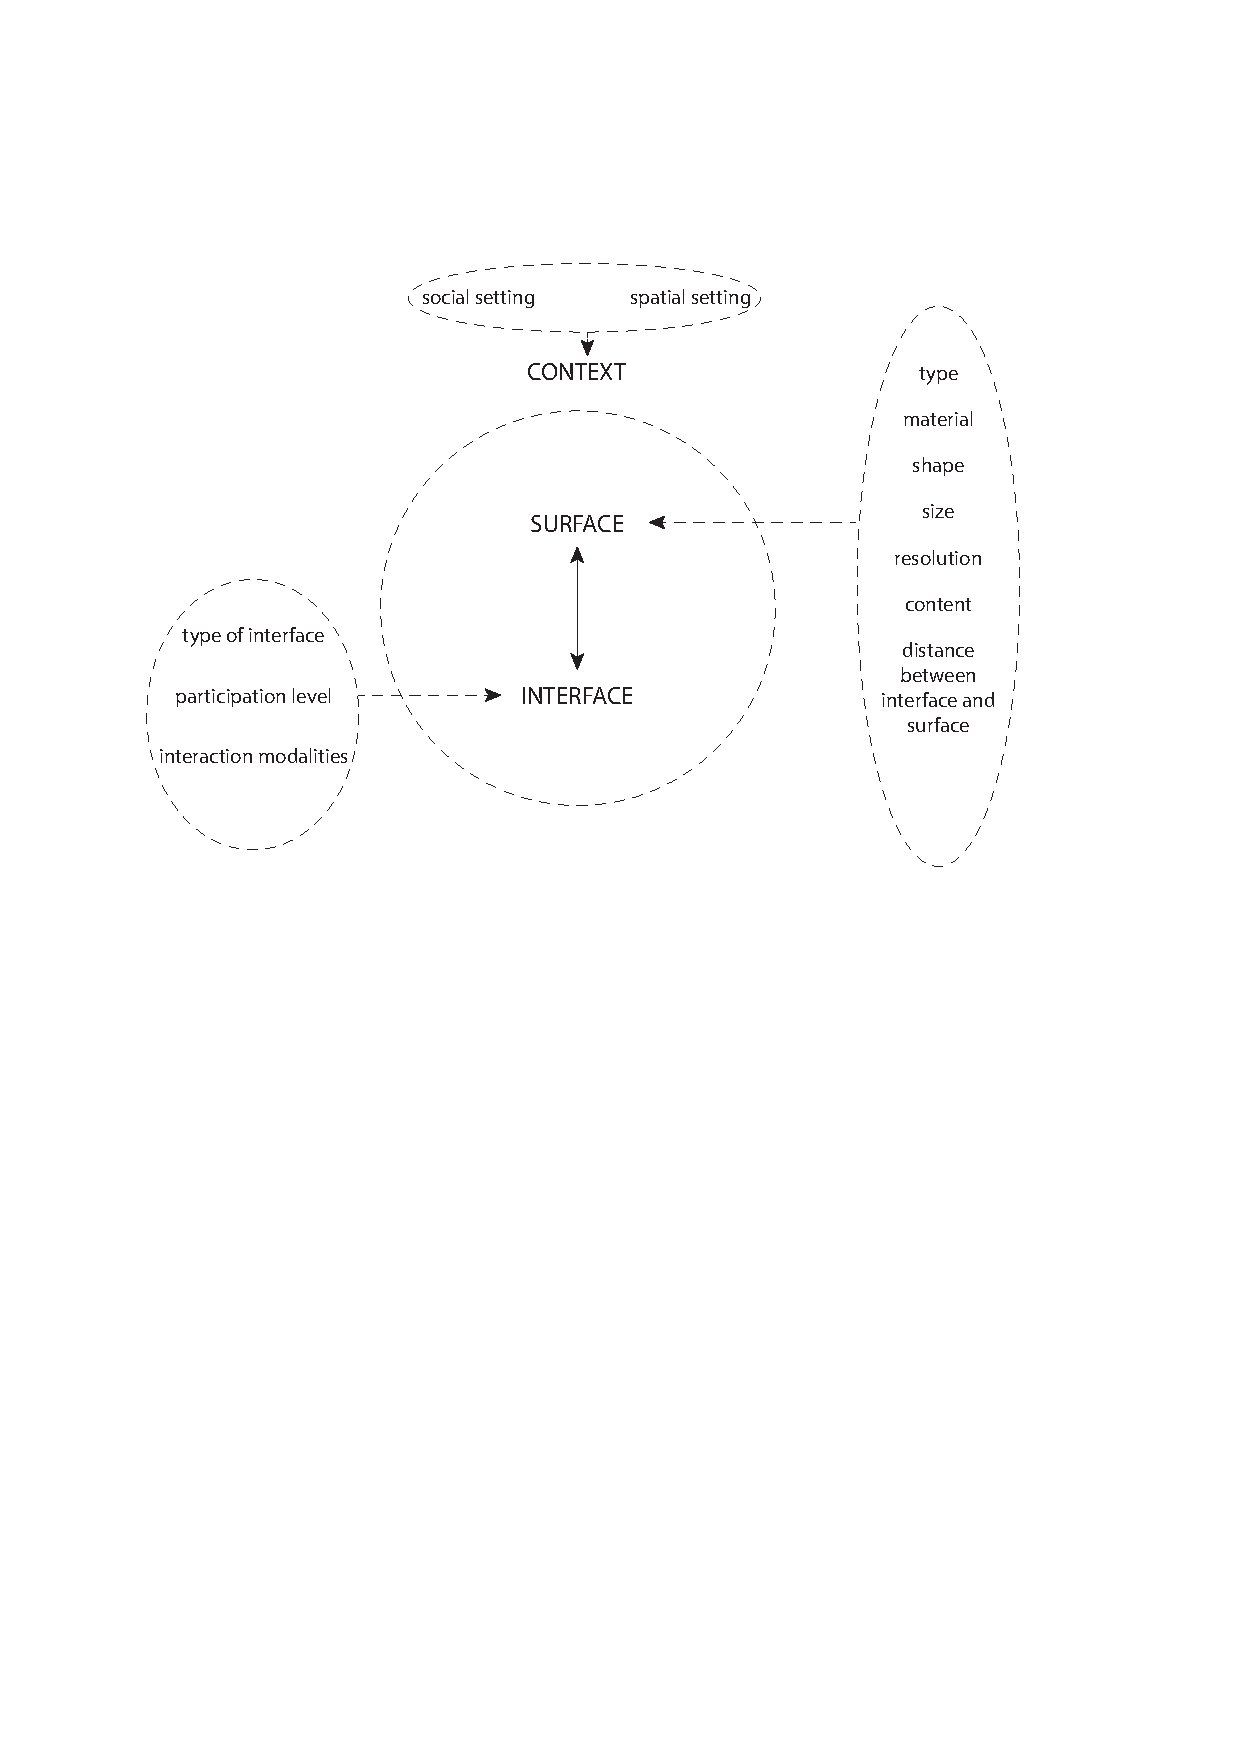
\includegraphics[width=\textwidth]{Illustrations/MAI_Framework.pdf}
\caption{Framework for Media Architectural Interfaces (MAI)}
\label{fig:MAI_Framework}
\end{figure}

\section{Taxonomy of Media Architectural Interfaces}

We introduce a taxonomy for the categorisation of MAI based on the triangular relationship between tangible \textit{Interfaces}, electronic \textit{Surfaces} and the \textit{Context}. Five exemplary media art projects are chosen, which were showcased during the CC Network events.
We have plotted the relevant information to gain a better understanding of the relation between the individual properties concerned with different electronic surfaces (\label{fig:CCN_Taxonomy}).
Large electronic surfaces amplify participants’ interactions through the tangible interfaces, which depend on technical properties of these surfaces such as type, shape, material, size and resolution of the surface. Both interfaces (tangible and non-tangible) are dependent on the given socio-spatial setting, for example on pedestrianised places, busy high streets or transport hubs. 
As a consequence, the distance between the tangible interface and the display can vary. 
Furthermore, when changing the properties within one of the three constituent elements (Surface, Interface or Context) the two other elements are directly affected. 

The properties of each constituent element are described in the following: Regarding the Interface, the characteristics for the \textit{level of participation} have been described by Fritsch and Brynskov as \textit{static, dynamic, reactive, interactive, participatory,} and \textit{communicative} and recently extended by Caldwell and Foth who added the terms \textit{performative} and \textit{controllable}.
The characteristics of the \textit{interaction modalities} originates from dimensions summarised by Müller et al. and uses the following interaction modalities: \textit{presence, body position, body posture, facial expression, gaze, speech, gestures, remote control, keys, touch} . 
This may also impact the distance between the Interface and the Surface. 
Being aware of these properties and their characteristics will help designers clarify the nature of interaction they want to design for.
The properties concerned with the Surface are mostly related to the technical details of large electronic surfaces, as described by Halskov and Ebsen.
They consist of \textit{type, material, shape, size} and \textit{resolution} but also of the \textit{type of content}. 
Each of these characteristics can impact the multi-layered spatial frameworks described above (i.e. Awareness Spaces, Actor Spaces, Action Spaces, Physical Spaces).
The Context refers to an understanding of the socio-spatial settings that are core properties, when locating a MAI. 
There is a huge difference when designing in the context of a pedestrianised court in the city (i.e. Medialab-Prado or Ars Electronica Center) or a busy high street such as the SESI Digital Gallery in São Paulo.
Although most of the characteristics aligned in the taxonomy describe the properties of the constituent elements (i.e. Surface, Interface, Context) from a technical point of view, they influence the multi-layered spatial frameworks (i.e. Awareness Spaces, Actor Spaces, Action Spaces, Physical Spaces) and consequently the MAI design space for interactions in the urban setting. 


In summary, it appears that the affordance of each of the described spaces has a strong impact on the presented studies and therefore need to be taken into account when designing for such interactive systems in the built environment. 
With this in mind, we return to our initial question: How to actually go about designing for an interaction with MAI? 
To help answering this question, we now introduce a taxonomy for the categorisation of MAI based on the triangular relationship between TUI, display and setting. 
We have plotted the relevant information of both design studies against each other to gain a better understanding of the relation between the individual properties.
In more detail, the properties of each constituent element will be described below:
\textbf{Interface: }The characteristics for the participation level have been described by Fritsch and Brynskov (2011) as (1) static, (2) dynamic, (3) reactive, (4) interactive, (5) participatory and (6) communicative and recently have been extended by Caldwell and Foth (2014), who added the terms (7) performative and (8) controllable.
The characteristics of the interaction modalities originate from dimensions summarised by Müller et al. (2010) and use the following interaction modalities:
(1) presence, (2) body position, (3) body posture, (4) facial expression, (5) gaze, (6) speech, (7) gestures, (8) remote control, (9) keys and (10) touch. 
This may also impact the distance between the interface and the display. 
Being aware of these properties and their characteristics will allow designers clarifying the nature of interaction they want to design for.
\textbf{Display: }These properties are mostly related to the technical details of large programmable displays as described by Halskov and Ebsen (2013). They consist of (1) type, (2) material, (3) shape, (4) size and (5) resolution but also of (6) the type of content. Each of these characteristics can impact the multilayered spatial frameworks described above (i.e. awareness, action, actor, physical).
\textbf{Context: }Understanding the socio-spatial settings as described in Sect. 2.1 are core properties when locating a MAI. As explained in this paper, here is a huge difference when designing in the context of a pedestrianised university court (i.e. VEIV London) or a busy high street (i.e. SCSD Sao Paulo).
Although most of the characteristics aligned in our taxonomy describe the properties of the constituent elements (i.e. display, interface, context) from a technical point of view, they influence the multilayered spatial frameworks (i.e. awareness, actor, action, physical) and consequently assist when designing MAI for interactions in urban space. 
Through understanding the effect of the single properties of each constituent element on the whole interactive system, designers may eventually be able to be fully aware of their design decisions.

\begin{figure}[htp]
\centering
\includegraphics[width=\textwidth]{Illustrations/CCN_Taxonomy.pdf}
\caption{Taxonomy for categorising Media Architectural Interfaces in five CC Network selected projects}
\label{fig:CCN_Taxonomy}
\end{figure}
In this chapter, we have introduced the notion of Media Architectural Interfaces (MAI) and highlighted its socio-spatial implications when designing interactive systems in urban space. In order to support this framework we displayed relevant projects in a taxonomy. 
Through understanding the effect of the single properties of each constituent element on the whole interactive system stakeholders, curators, artists, designers and architects may eventually be more aware of their design decisions and their implications.

